% Define the document type and font size
\documentclass[12pt]{article}

\usepackage[spanish]{babel} % Package for the Spanish language
\usepackage[utf8]{inputenc} % Package for UTF-8 character encoding
\usepackage{geometry} % Package to configure document margins
\usepackage{listings} % Package to include source code in the document
\usepackage{xcolor} % Package to define colors
\usepackage{fancyhdr} % Package to customize headers and footers
\usepackage{amsmath} % Package for advanced mathematical symbols and environments
\usepackage{amssymb} % Package for additional mathematical symbols
\usepackage{graphicx} % Package to include graphics
\usepackage{multirow} % Package to create tables with multiple rows
\usepackage{ragged2e} % Package to justify text
\usepackage{pdflscape} % Package to create landscape pages

\setlength{\parskip}{1em} % Space between paragraphs
\setlength{\parindent}{0pt} % Without indentation for paragraphs

% Definition of colors for source code
\definecolor{KEYWORDS}{HTML}{0000ff}
\definecolor{COMMENTS}{HTML}{888888}
\definecolor{STRINGS}{HTML}{ff0000}

% Configuration of the listings environment to display source code
\lstset{
	frame=shadowbox,
	language=c++,
	aboveskip=3mm,
	belowskip=3mm,
	xleftmargin=10mm,
	xrightmargin=10mm,
	showstringspaces=false,
	columns=flexible,
	basicstyle={\small\ttfamily},
	numbers=left,
	numberstyle=\tiny\color{COMMENTS},
	keywordstyle=\color{KEYWORDS},
	commentstyle=\color{COMMENTS},
	stringstyle=\color{STRINGS},
	breaklines=true,
	breakatwhitespace=true,
	tabsize=4
}

% Configuration of document margins
\geometry{
	a4paper,
	left=25mm,
	right=25mm,
	top=25mm,
	bottom=25mm
}

\title{Proyecto Cacerola - Modelado del Dominio} % Document title
\author{Druxorey} % Document author
\date{\today} % Document date

\begin{document}

\begin{titlepage}
	\centering
	\vspace{1cm}
	{\large {Universidad Central de Venezuela}\par}
	{\large {Facultad de Ciencias}\par}
	{\large {Escuela de Computación}\par}
	{\large {Ingeniería de Software}\par}
	\vspace{6cm}
	{\LARGE \textbf{Disciplina de Requisitos}\par}
	\vspace{0.25cm}
	{\Large \textbf{Entrega 2}\par}
	\vfill
	\begin{flushleft}
		{\large Profesor: Marcel Castro\par\vspace{-0.5em}}
		{\large Sección: C2\par\vspace{-0.5em}}
		{\large Equipo \#2\par\vspace{-1em}}
		\begin{itemize}
			\item Guillermo Galavís\vspace{-0.5em}
			\item José Apure\vspace{-0.5em}
			\item Renzo Morales\vspace{-0.5em}
			\item Luis David Lima\vspace{-0.5em}
		\end{itemize}
	\end{flushleft}
	\vspace{0.5cm}
	\centering
	{\large \today\par}
\end{titlepage}

\section{Visión del Producto}

\vspace{1cm}
\begin{table}[htbp]
	\centering
	\begin{tabular}{|p{3.5cm}|p{3.5cm}|p{3.5cm}|p{3.5cm}|}
	\hline
	\textbf{Nombre Clave}			  & \multicolumn{3}{p{8cm}|}{\textbf{Frase Representativa}}												  \\ \hline
	\multicolumn{1}{|p{3.5cm}|}{MiComedorUCV} & \multicolumn{3}{p{8cm}|}{Sistema para la gestión eficiente del comedor universitario}					\\ \cline{1-4}
	\textbf{Grupo de Usuarios}		 & \multicolumn{1}{p{3.5cm}|}{\textbf{Necesidades}} & \multicolumn{1}{p{3.5cm}|}{\textbf{Producto}} & \textbf{Valor} \\ \cline{1-4}
	\begin{tabular}[c]{@{}p{3.5cm}@{}}- Estudiantes pertenecientes a la Universidad Central de Venezuela.\\ - Personal Docente.\\ - Personal Administrativo.\\ - Personal Obrero.\end{tabular} &
	\begin{tabular}[c]{@{}p{3.5cm}@{}}- Consultar el menú semanal disponible.\\ - Acceder al comedor en turnos asignados.\\ - Conocer los horarios de los turnos de comida.\\ - Obtener reportes del consumo y demanda.\\ - Gestionar los insumos y menús semanalmente.\\ - Evitar largas filas al ingresar al comedor.\\ - Saber si el usuario tiene un cupo en un turno específico.\end{tabular} &
	\begin{tabular}[c]{@{}p{3.5cm}@{}}- Permitir consultar el menú semanal.\\ - Gestionar la asignación de turnos y cupos.\\ - Visualizar la información de turnos de comida.\\ - Generar reportes de consumo y demanda.\\ - Administrar los insumos y la planificación de menús.\\ - Validar la reserva de cupos por usuario.\\ - Registrar nuevos usuarios (estudiantes, docentes, administrativos, obreros).\\ - Controlar el acceso a los turnos programados.\end{tabular} &
	\begin{tabular}[c]{@{}p{3.5cm}@{}}- Acceso ágil y sin demoras al comedor.\\ - Mayor control y planificación de sus comidas.\\ - Experiencia de servicio mejorada y más cómoda.\\ - Optimización de la gestión de recursos e insumos.\\ - Mejor control del inventario y desperdicio de alimentos.\\ - Mejora en la eficiencia operativa del comedor.\end{tabular} \\ \hline
	\end{tabular}
\end{table}

\pagebreak

\section{Diagrama de Casos de Uso}
\vspace{1cm}
\begin{center}
	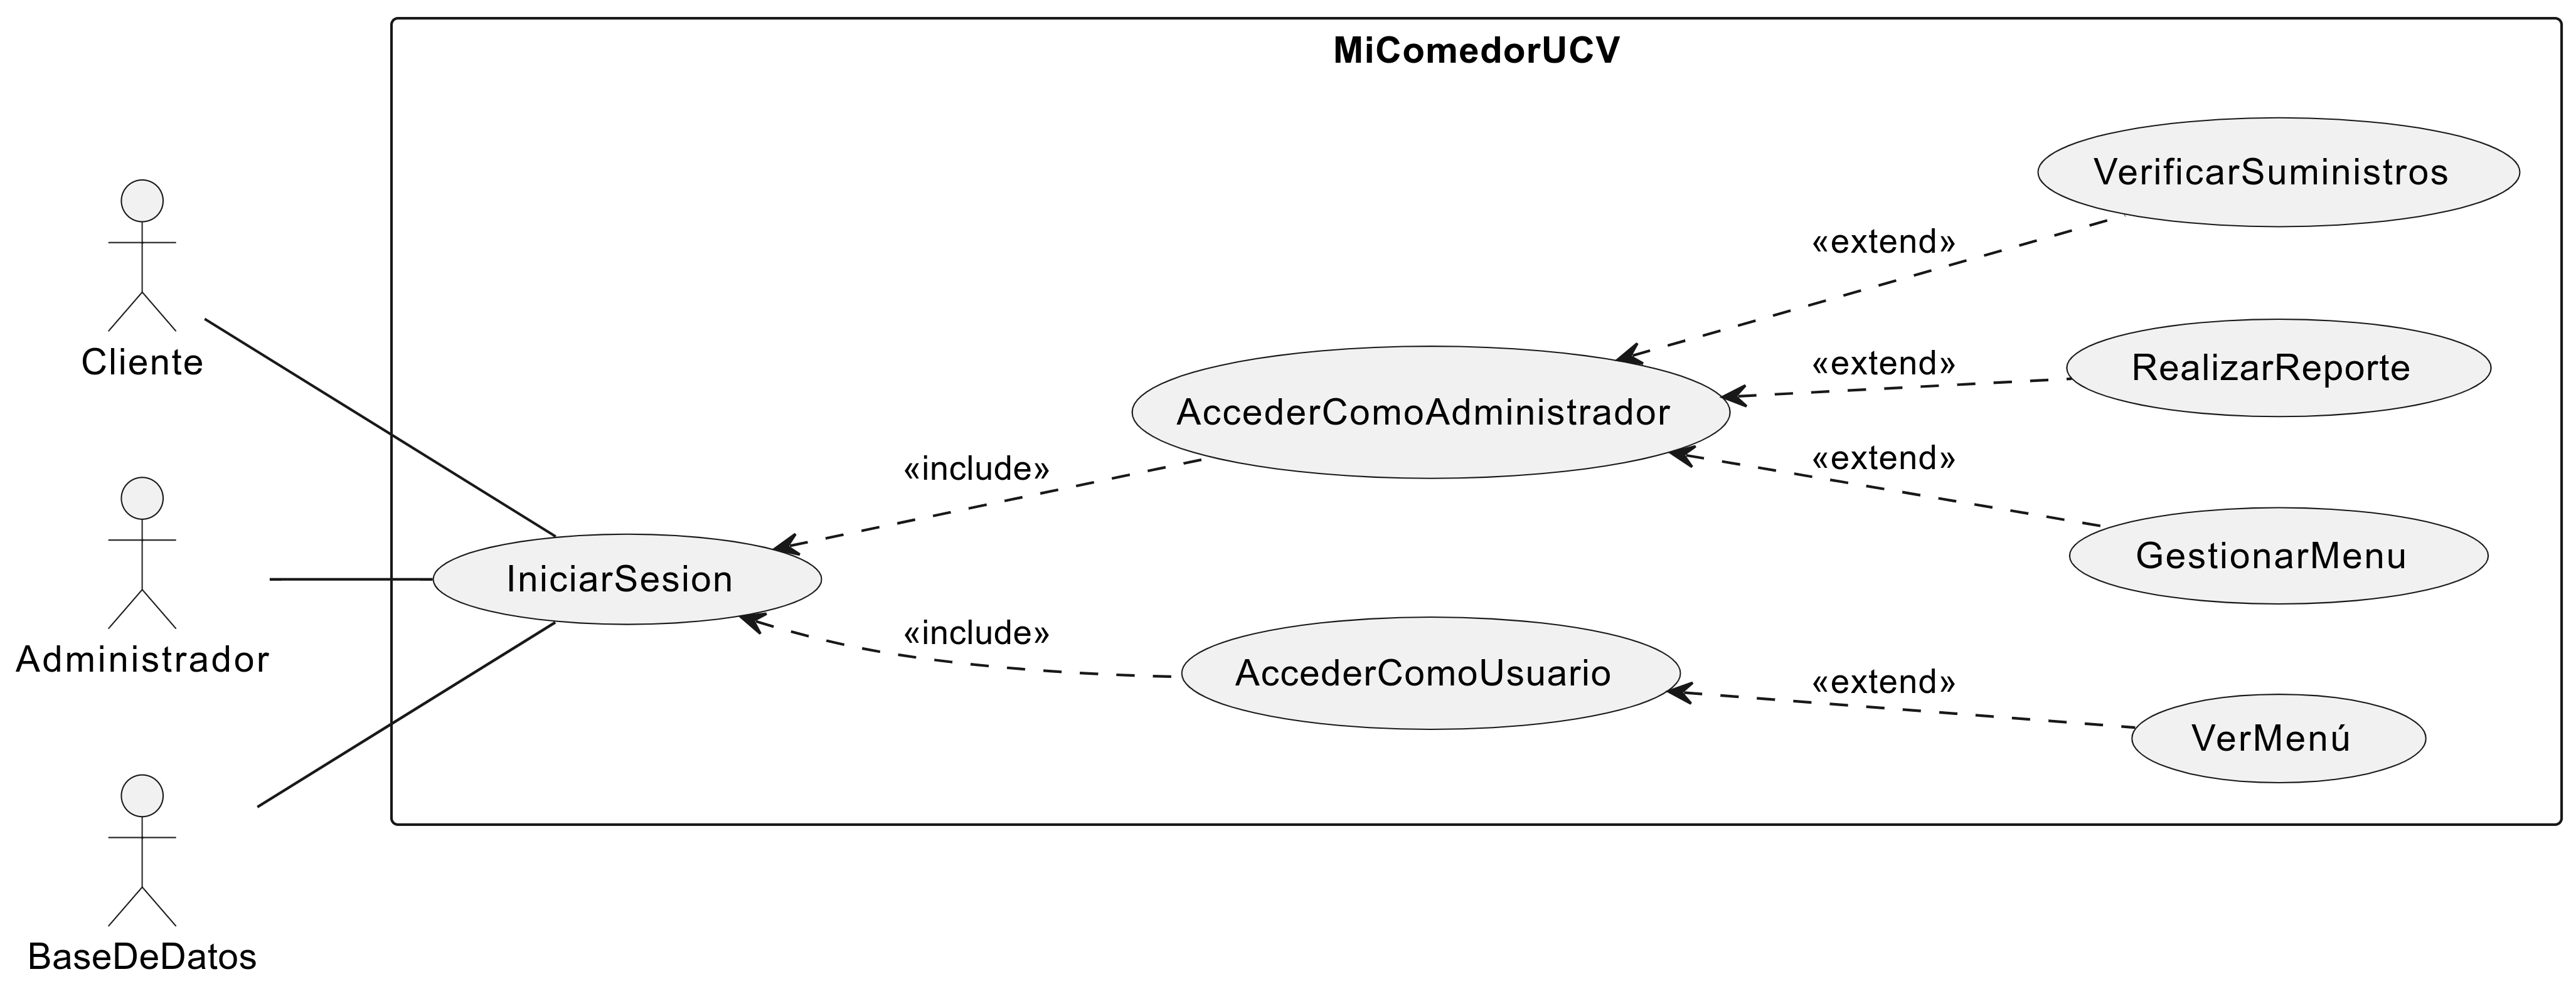
\includegraphics[width=12cm]{Requirements Discipline - Uses Cases Diagram.png}
\end{center}

\pagebreak

\section{Lista de Casos de Uso Prioritario}

\subsection*{Lista de Casos de Uso}

\begin{itemize}
	\item \textbf{Iniciar Sesión}: Este caso de uso permite a los usuarios (\textbf{usuarios} y \textbf{administradores}) acceder al sistema. Es el punto de entrada principal que autentica al usuario y le concede acceso a las funcionalidades correspondientes a su rol. Es un proceso fundamental para la seguridad y la usabilidad del sistema.

	\item \textbf{Registrarse}: Permite a los nuevos \textbf{usuarios} crear una cuenta en el sistema. Se considera una extensión de «Iniciar Sesión» porque un registro exitoso suele llevar al inicio de sesión automático o a la necesidad de iniciar sesión.

	\item \textbf{Ver Turnos}: La funcionalidad central para los \textbf{usuarios}, que les permite a los \textbf{usuarios} conocer los horarios y la disponibilidad de los turnos para el comedor. Esto es esencial para que los usuarios puedan planificar su visita y asegurar su lugar, especialmente en un comedor que maneja horarios específicos o capacidad limitada.

	\item \textbf{Ver Menú}: Permite consultar los platos, bebidas y otras ofertas disponibles en el comedor. Este caso de uso es la razón principal por la que un usuario usaría la aplicación, proporcionando la información necesaria para decidir qué consumir. Es un caso de uso que se incluye dentro de «Ver Turnos».

	\item \textbf{Gestionar Menú}: Este caso de uso es exclusivo para el \textbf{administrador} y le permite realizar todas las operaciones relacionadas con el menú del comedor: añadir nuevos platos, modificar los existentes (precio, descripción, disponibilidad) o eliminarlos. Es vital para mantener la información del menú actualizada y reflejar la oferta real del comedor.

	\item \textbf{Gestionar Turnos}: También exclusivo del \textbf{administrador}, esta funcionalidad le permite crear, modificar o eliminar los turnos disponibles en el comedor. Esto incluye establecer la duración de los turnos, la capacidad de cada uno, y cualquier otra regla asociada, lo cual es crucial para la organización y eficiencia del servicio.

	\item \textbf{Realizar Reporte}: Un caso de uso para el \textbf{administrador} que le permite generar informes sobre diversos aspectos del comedor, como el uso del servicio, la afluencia de usuarios en ciertos turnos, la popularidad de los platos, etc. Estos reportes son herramientas clave para la toma de decisiones, la optimización de recursos y la mejora continua del servicio.

	\item \textbf{Verificar Suministros}: Este caso de uso también es para el \textbf{administrador} y le permite llevar un control y gestión de los inventarios de ingredientes y suministros necesarios para la operación del comedor.
\end{itemize}

\pagebreak

\subsection*{Explicación de los Usuarios}

\begin{itemize}
	\item \textbf{Usuario}: Este es el usuario final del comedor. Su interacción principal con el sistema se centra en la consulta de información y la preparación para hacer uso del servicio. El \textbf{usuario} puede \textbf{ver el turno} (lo que implica también \textbf{ver los menús}) y tiene la capacidad de \textbf{registrarse} e \textbf{iniciar sesión} para acceder a estas funcionalidades. Su rol es fundamental para la operación del comedor, ya que son los beneficiarios directos del servicio.

	\item \textbf{Administrador}: Este usuario tiene un rol de gestión y control sobre el sistema y la operación del comedor. El \textbf{administrador} es el encargado de mantener la información actualizada y de supervisar el funcionamiento del servicio. Sus responsabilidades incluyen \textbf{iniciar sesión}, \textbf{gestionar el menú} (actualizar los platos), \textbf{gestionar los turnos} (establecer la disponibilidad y capacidad), \textbf{realizar reportes} (para análisis y toma de decisiones), y \textbf{verificar los suministros} (para el control de inventario). El administrador asegura que el sistema y el comedor funcionen de manera eficiente.

	\item \textbf{Base De Datos de la UCV}: Aunque no es un usuario humano, este actor representa el \textbf{sistema de información centralizado de la Universidad Central de Venezuela}. Esta base de datos contiene los registros de todos los \textbf{estudiantes, personal docente, administrativo y obrero} que forman parte de la institución.
\end{itemize}

\pagebreak
\section{Especificación de Casos de Uso Prioritarios}

\vspace{1cm}
\begin{table}[htbp]
	\centering
	\begin{tabular}{|l|lll|}
	\hline
	\textbf{Caso de Uso} & \multicolumn{3}{l|}{CU \#0 Iniciar sesión} \\ \hline
	\textbf{Versión} & \multicolumn{1}{l|}{1} & \multicolumn{1}{l|}{Release} & 31/5/2025 \\ \hline
	\textbf{Estado} & \multicolumn{1}{l|}{Presentando} & \multicolumn{1}{l|}{Autor} & José Apure \\ \hline
	\textbf{Actor/es} & \multicolumn{3}{l|}{Usuario, Administrador, Base de Datos} \\ \hline
	\textbf{Flujo Normal} & \multicolumn{3}{l|}{\begin{tabular}[c]{@{}l@{}}1.El cliente selecciona la opción de iniciar sesión.\\ 2. El sistema arroja un formulario de inicio de sesión.\\ 3. El usuario ingresa sus datos (número de cédula y \\ contraseña), y da clic en el botón de iniciar sesión.\\ 4. Dependiendo de los datos, el sistema lo deja acceder \\ a la parte de clientes o de administradores.\end{tabular}} \\ \hline
	\multirow{2}{*}{\textbf{Flujo Alternativo}} & \multicolumn{1}{l|}{A1} & \multicolumn{2}{l|}{\begin{tabular}[c]{@{}l@{}}4. Si los datos no coinciden, el sistema\\ arroja un error.\\ 5. Se regresa al paso 1.\end{tabular}} \\ \cline{2-4} 
	& \multicolumn{1}{l|}{A2} & \multicolumn{2}{l|}{\begin{tabular}[c]{@{}l@{}}4. Si el usuario no está registrado, el\\ sistema arroja un error.\\ 5. Se regresa al paso 1.\end{tabular}} \\ \hline
	\textbf{\begin{tabular}[c]{@{}l@{}}Requisitos No\\ Funcionales\end{tabular}} & \multicolumn{3}{l|}{Sistema de Inicio de Sesión} \\ \hline
	\end{tabular}
\end{table}

\begin{table}[htbp]
	\centering
	\begin{tabular}{|l|lll|}
	\hline
	\textbf{Caso de Uso} & \multicolumn{3}{l|}{CU \#1 Realizar Pedido} \\ \hline
	\textbf{Versión} & \multicolumn{1}{l|}{1} & \multicolumn{1}{l|}{Release} & 31/5/2025  \\ \hline
	\textbf{Estado} & \multicolumn{1}{l|}{Aprobado} & \multicolumn{1}{l|}{Autor} & José Apure \\ \hline
	\textbf{Actor/es} & \multicolumn{3}{l|}{Cliente} \\ \hline
	\textbf{Flujo Normal} & \multicolumn{3}{l|}{\begin{tabular}[c]{@{}l@{}}1. El usuario hace clic en la opción de realizar pedido.\\ 2. Ingresa los datos del pedido a realizar.\\ 3. Realiza el pago a través de un pago móvil o \\ transferencia bancaria.\\ 4. Va al local para ingerir el platillo.\end{tabular}} \\ \hline
	\multirow{2}{*}{\textbf{Flujo Alternativo}} & \multicolumn{1}{l|}{A1} & \multicolumn{2}{l|}{\begin{tabular}[c]{@{}l@{}}2. El usuario ingresa los datos del pedido.\\ 3. El sistema arroja un error, ya que no \\ esta disponible el platillo seleccionado.\\ 4. Se devuelve al paso 2.\end{tabular}} \\ \cline{2-4} 
	& \multicolumn{1}{l|}{A2} & \multicolumn{2}{l|}{\begin{tabular}[c]{@{}l@{}}3. El usuario escoge la opción de pagar \\ en efectivo.\\ 4. Va al local a ingerir el platillo\\ 5. Al terminar, paga en una caja.\end{tabular}} \\ \hline
	\textbf{\begin{tabular}[c]{@{}l@{}}Requisitos No\\ Funcionales\end{tabular}} & \multicolumn{3}{l|}{\begin{tabular}[c]{@{}l@{}}Sistema de pago interbancario.\\ Sistema de cajas de pago.\end{tabular}} \\ \hline
	\end{tabular}
\end{table}

\begin{table}[htbp]
	\centering
	\begin{tabular}{|l|lll|}
	\hline
	\textbf{Caso de Uso} & \multicolumn{3}{l|}{CU \#2 Ver menú} \\ \hline
	\textbf{Versión} & \multicolumn{1}{l|}{1} & \multicolumn{1}{l|}{Release} & 31/5/2025 \\ \hline
	\textbf{Estado} & \multicolumn{1}{l|}{Aprobado} & \multicolumn{1}{l|}{Autor} & José Apure \\ \hline
	\textbf{Actor/es} & \multicolumn{3}{l|}{Cliente, Administrador.} \\ \hline
	\textbf{Flujo Normal} & \multicolumn{3}{l|}{\begin{tabular}[c]{@{}l@{}}1. El usuario hace clic en la opción de ver menú.\\ 2. Se muestra el menú del día.\\ 3. El usuario hace clic en salir.\end{tabular}} \\ \hline
	\multirow{2}{*}{\textbf{Flujo Alternativo}} & \multicolumn{1}{l|}{A1} & \multicolumn{2}{l|}{\begin{tabular}[c]{@{}l@{}}2. Se muestra un error que dice que no\\ hay menú disponible.\\ 3. El sistema sale de la opción automáticamente\\ a los 30 segundos de mostrar el mensaje.\end{tabular}} \\ \cline{2-4} 
	& \multicolumn{1}{l|}{A2} & \multicolumn{2}{l|}{\begin{tabular}[c]{@{}l@{}}3. Los administradores tiene la opción de\\ modificar el menú, su botón esta al lado del\\ botón de salir.\\ 4. Se hace clic en el botón de modificar menú.\\ 5. Se despliega una lista que contiene una\\ imagen, el nombre del platillo, y una corta\\ descripción del mismo.\\ 6. Al terminar, se presiona el botón de\\ guardar cambios.\\ 7. Se vuelve al paso 2.\end{tabular}} \\ \hline
	\textbf{\begin{tabular}[c]{@{}l@{}}Requisitos No\\ Funcionales\end{tabular}} & \multicolumn{3}{l|}{} \\ \hline
	\end{tabular}
\end{table}

\begin{table}[htbp]
	\centering
	\begin{tabular}{|l|lll|}
	\hline
	\textbf{Caso de Uso} & \multicolumn{3}{l|}{CU \#3 Realizar reporte} \\ \hline
	\textbf{Versión} & \multicolumn{1}{l|}{1} & \multicolumn{1}{l|}{Release} & 31/5/2025 \\ \hline
	\textbf{Estado} & \multicolumn{1}{l|}{Aprobado} & \multicolumn{1}{l|}{Autor} & José Apure \\ \hline
	\textbf{Actor/es} & \multicolumn{3}{l|}{Administrador.} \\ \hline
	\textbf{Flujo Normal} & \multicolumn{3}{l|}{\begin{tabular}[c]{@{}l@{}}1. El administrador hace clic en el botón de realizar reporte.\\ 2. Se despliega una lista con todos los reportes realizados.\\ 3. El administrador hace clic en realizar nuevo reporte.\\ 4. Al terminar de redactar el reporte, el administrador\\ hace clic en la opción de archivar reporte.\\ 5. Se archiva el reporte y se vuelve al paso 2.\end{tabular}} \\ \hline
	\multirow{3}{*}{\textbf{Flujo Alternativo}} & \multicolumn{1}{l|}{A1} & \multicolumn{2}{l|}{\begin{tabular}[c]{@{}l@{}}2. El sistema muestra un mensaje que dice\\ “lista vacía”, y se muestra el botón de realizar\\ nuevo reporte más grande de lo usual.\\ 3. Se continua con el paso 3 de manera normal.\end{tabular}} \\ \cline{2-4} 
	& \multicolumn{1}{l|}{A2} & \multicolumn{2}{l|}{\begin{tabular}[c]{@{}l@{}}4. Se tiene la opción de cancelar el reporte.\\ 5. No se archiva el reporte, se muestra un mensaje\\ que dice “reporte cancelado”, y se regresa al paso 2.\end{tabular}} \\ \cline{2-4} 
	& \multicolumn{1}{l|}{A3} & \multicolumn{2}{l|}{\begin{tabular}[c]{@{}l@{}}2. Se tiene la opción de salir de la lista.\\ 3. El administrador hace clic en salir.\\ 4. El sistema vuelve al menú principal.\end{tabular}} \\ \hline
	\textbf{\begin{tabular}[c]{@{}l@{}}Requisitos No\\ Funcionales\end{tabular}} & \multicolumn{3}{l|}{} \\ \hline
	\end{tabular}
\end{table}

\begin{table}[htbp]
	\centering
	\begin{tabular}{|l|lll|}
	\hline
	\textbf{Caso de Uso} & \multicolumn{3}{l|}{CU \#4 Verificar suministros} \\ \hline
	\textbf{Versión} & \multicolumn{1}{l|}{1} & \multicolumn{1}{l|}{Release} & 31/5/2025 \\ \hline
	\textbf{Estado} & \multicolumn{1}{l|}{Aprobado} & \multicolumn{1}{l|}{Autor} & José Apure \\ \hline
	\textbf{Actor/es} & \multicolumn{3}{l|}{Administrador.} \\ \hline
	\textbf{Flujo Normal} & \multicolumn{3}{l|}{\begin{tabular}[c]{@{}l@{}}1. El administrador hace clic en el botón de “gestión de \\ suministros”.\\ 2. Se despliega una lista con todos los suministros,\\ conteniendo nombre, descripción y cantidad de cada uno.\\ 3. El administrador modifica las cantidades de los\\ suministros.\\ 4. Al finalizar, se hace clic en el botón de “guardar\\ cambios”.\\ 5. Se aplican los cambios y se vuelve al paso 2.\end{tabular}} \\ \hline
	\multirow{3}{*}{\textbf{Flujo Alternativo}} & \multicolumn{1}{l|}{A1} & \multicolumn{2}{l|}{\begin{tabular}[c]{@{}l@{}}3. El administrador tiene la opción de agregar\\  o eliminar suministros.\\ 4. Se continua con el paso 4 de forma normal.\end{tabular}} \\ \cline{2-4} 
	& \multicolumn{1}{l|}{A2} & \multicolumn{2}{l|}{\begin{tabular}[c]{@{}l@{}}2. El sistema no muestra la lista, sino un\\ mensaje de “sin suministros”.\\ 3. Se continua con el paso 3 de forma normal.\end{tabular}} \\ \cline{2-4} 
	& \multicolumn{1}{l|}{A3} & \multicolumn{2}{l|}{\begin{tabular}[c]{@{}l@{}}2. Se tiene la opción de salir de la lista.\\ 3. El administrador hace clic en salir.\\ 4. El sistema vuelve al menú principal.\end{tabular}} \\ \hline
	\textbf{\begin{tabular}[c]{@{}l@{}}Requisitos No\\ Funcionales\end{tabular}} & \multicolumn{3}{l|}{} \\ \hline
	\end{tabular}
\end{table}

\begin{table}[htbp]
	\centering
	\begin{tabular}{|l|lll|}
	\hline
	\textbf{Caso de Uso} & \multicolumn{3}{l|}{CU \#5 Ver Turnos} \\ \hline
	\textbf{Versión} & \multicolumn{1}{l|}{1} & \multicolumn{1}{l|}{Release} & 31/5/2025 \\ \hline
	\textbf{Estado} & \multicolumn{1}{l|}{Aprobado} & \multicolumn{1}{l|}{Autor} & José Apure \\ \hline
	\textbf{Actor/es} & \multicolumn{3}{l|}{Usuario} \\ \hline
	\textbf{Flujo Normal} & \multicolumn{3}{l|}{\begin{tabular}[c]{@{}l@{}}1.El cliente hace clic en la opción de ver turnos.\\ 2.El sistema le despliega los turnos disponibles, junto con\\ la hora en la que está disponible y su respectivo menú.\\ 3.El cliente selecciona la hora a la que desea ir.\\ 4.Se le genera un qr para identificarse en el comedor.\end{tabular}} \\ \hline
	\textbf{Flujo Alternativo} & \multicolumn{1}{l|}{A1} & \multicolumn{2}{l|}{\begin{tabular}[c]{@{}l@{}}2. El sistema muestra un mensaje que indica\\ que no hay turnos disponibles para ese día.\\ 3. El sistema le permite ver los turnos del\\ día siguiente.\\ 4. Vuelve al paso 2.\end{tabular}} \\ \hline
	\textbf{\begin{tabular}[c]{@{}l@{}}Requisitos No\\ Funcionales\end{tabular}} & \multicolumn{3}{l|}{Sistema de gestión de turnos.} \\ \hline
	\end{tabular}
\end{table}

\begin{table}[htbp]
	\centering
	\begin{tabular}{|l|lll|}
	\hline
	\textbf{Caso de Uso} & \multicolumn{3}{l|}{CU \#6 Gestionar Turnos} \\ \hline
	\textbf{Versión} & \multicolumn{1}{l|}{1} & \multicolumn{1}{l|}{Release} & 31/5/2025 \\ \hline
	\textbf{Estado} & \multicolumn{1}{l|}{Aprobado} & \multicolumn{1}{l|}{Autor} & José Apure \\ \hline
	\textbf{Actor/es} & \multicolumn{3}{l|}{Usuario} \\ \hline
	\textbf{Flujo Normal} & \multicolumn{3}{l|}{\begin{tabular}[c]{@{}l@{}}1.El administrador hace clic en la opción de gestionar turnos.\\ 2.El sistema le muestra los turnos disponibles hasta ese\\ momento y le da la opción de agregar o modificar turno.\\ 3.El administrador le da a la opción de agregar turno.\\ 4.El administrador llena los campos de horario y\\ menú disponible.\\ 5.El administrador hace clic en la opción de guardar cambios.\\ 6.Se devuelve al paso 2 con los cambios realizados.\end{tabular}} \\ \hline
	\textbf{Flujo Alternativo} & \multicolumn{1}{l|}{A1} & \multicolumn{2}{l|}{\begin{tabular}[c]{@{}l@{}}2. El administrador hace clic en modificar un turno.\\ 3. El administrador cambia los datos de horario\\ y/o menú.\\ 4. El administrador hace clic en guardar cambios.\\ 5. Se devuelve al paso 2 con los cambios realizados.\end{tabular}} \\ \hline
	& \multicolumn{1}{l|}{A2} & \multicolumn{2}{l|}{\begin{tabular}[c]{@{}l@{}}5. El administrador da clic en la opción de cancelar.\\ 6. Se devuelve al paso 2 sin realizar ningún cambio.\end{tabular}} \\ \hline
	\textbf{\begin{tabular}[c]{@{}l@{}}Requisitos No\\ Funcionales\end{tabular}} & \multicolumn{3}{l|}{Sistema de gestión de turnos.} \\ \hline
	\end{tabular}
\end{table}

\begin{table}[htbp]
	\centering
	\begin{tabular}{|l|lll|}
	\hline
	\textbf{Caso de Uso} & \multicolumn{3}{l|}{CU \#7 Registrarse} \\ \hline
	\textbf{Versión} & \multicolumn{1}{l|}{1} & \multicolumn{1}{l|}{Release} & 31/5/2025 \\ \hline
	\textbf{Estado} & \multicolumn{1}{l|}{Aprobado} & \multicolumn{1}{l|}{Autor} & José Apure \\ \hline
	\textbf{Actor/es} & \multicolumn{3}{l|}{Cliente (generalizado).} \\ \hline
	\textbf{Flujo Normal} & \multicolumn{3}{l|}{\begin{tabular}[c]{@{}l@{}}1.El cliente selecciona la opción de registrarse.\\ 2.El sistema muestra una interfaz de registro.\\ 3.El cliente ingresa sus datos (correo electrónico,\\ número de cédula, y contraseña).\\ 4.El cliente da clic en la opción de registrarse.\\ 5.El sistema lo registra en la base de datos y lo deja entrar.\end{tabular}} \\ \hline
	\textbf{Flujo Alternativo} & \multicolumn{1}{l|}{A1} & \multicolumn{2}{l|}{\begin{tabular}[c]{@{}l@{}}5. El sistema detecta que el usuario ya está\\ registrado, se lo notifica con un mensaje de \\ “cliente registrado”\\ 6. Se devuelve la paso 1.\end{tabular}} \\ \hline
	& \multicolumn{1}{l|}{A2} & \multicolumn{2}{l|}{\begin{tabular}[c]{@{}l@{}}4. El cliente da clic en cancelar.\\ 5. El sistema cancela el registro y se devuelve\\ al paso 1.\end{tabular}} \\ \hline
	\textbf{\begin{tabular}[c]{@{}l@{}}Requisitos No\\ Funcionales\end{tabular}} & \multicolumn{3}{l|}{Sistema de registro.} \\ \hline
	\end{tabular}
\end{table}

\pagebreak

\begin{landscape}
	\section{Diagrama de Contexto}
	\vspace{1cm}
	\begin{center}
		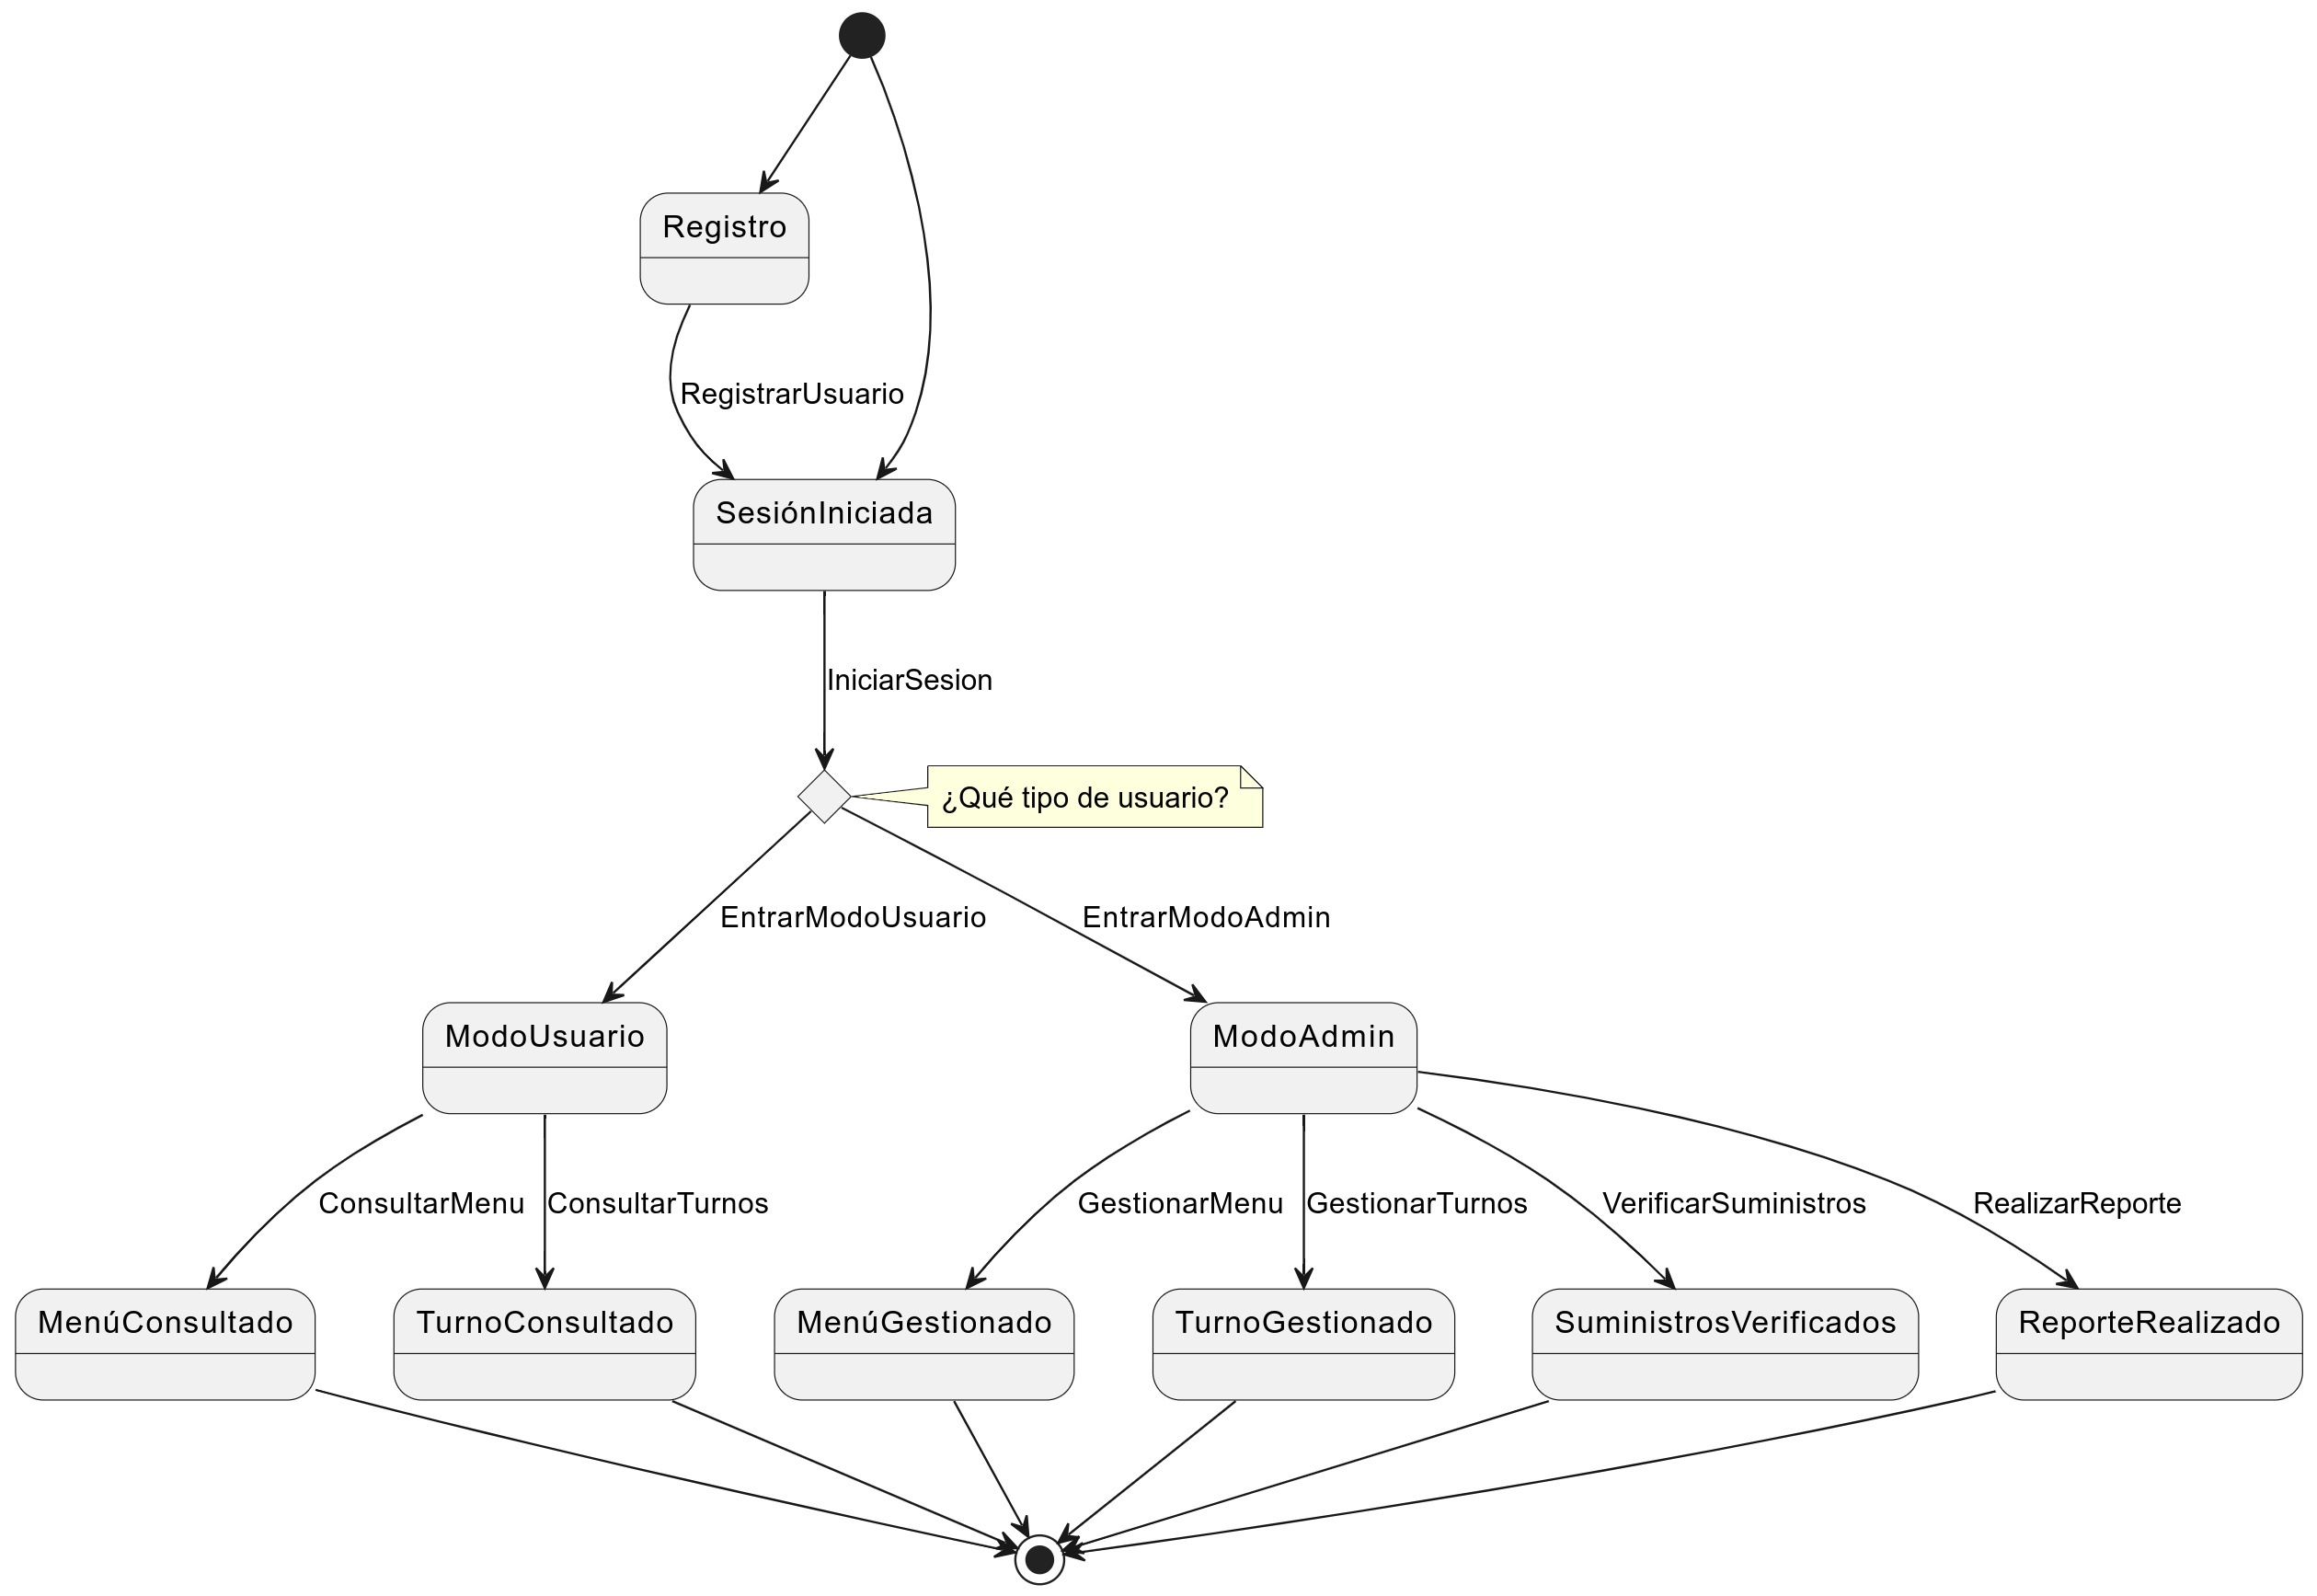
\includegraphics[width=19cm]{Requirements Discipline - Context Diagram.png}
	\end{center}
\end{landscape}

\pagebreak

\section{Prototipo de Interfaz}
\vspace{1cm}
\begin{center}
	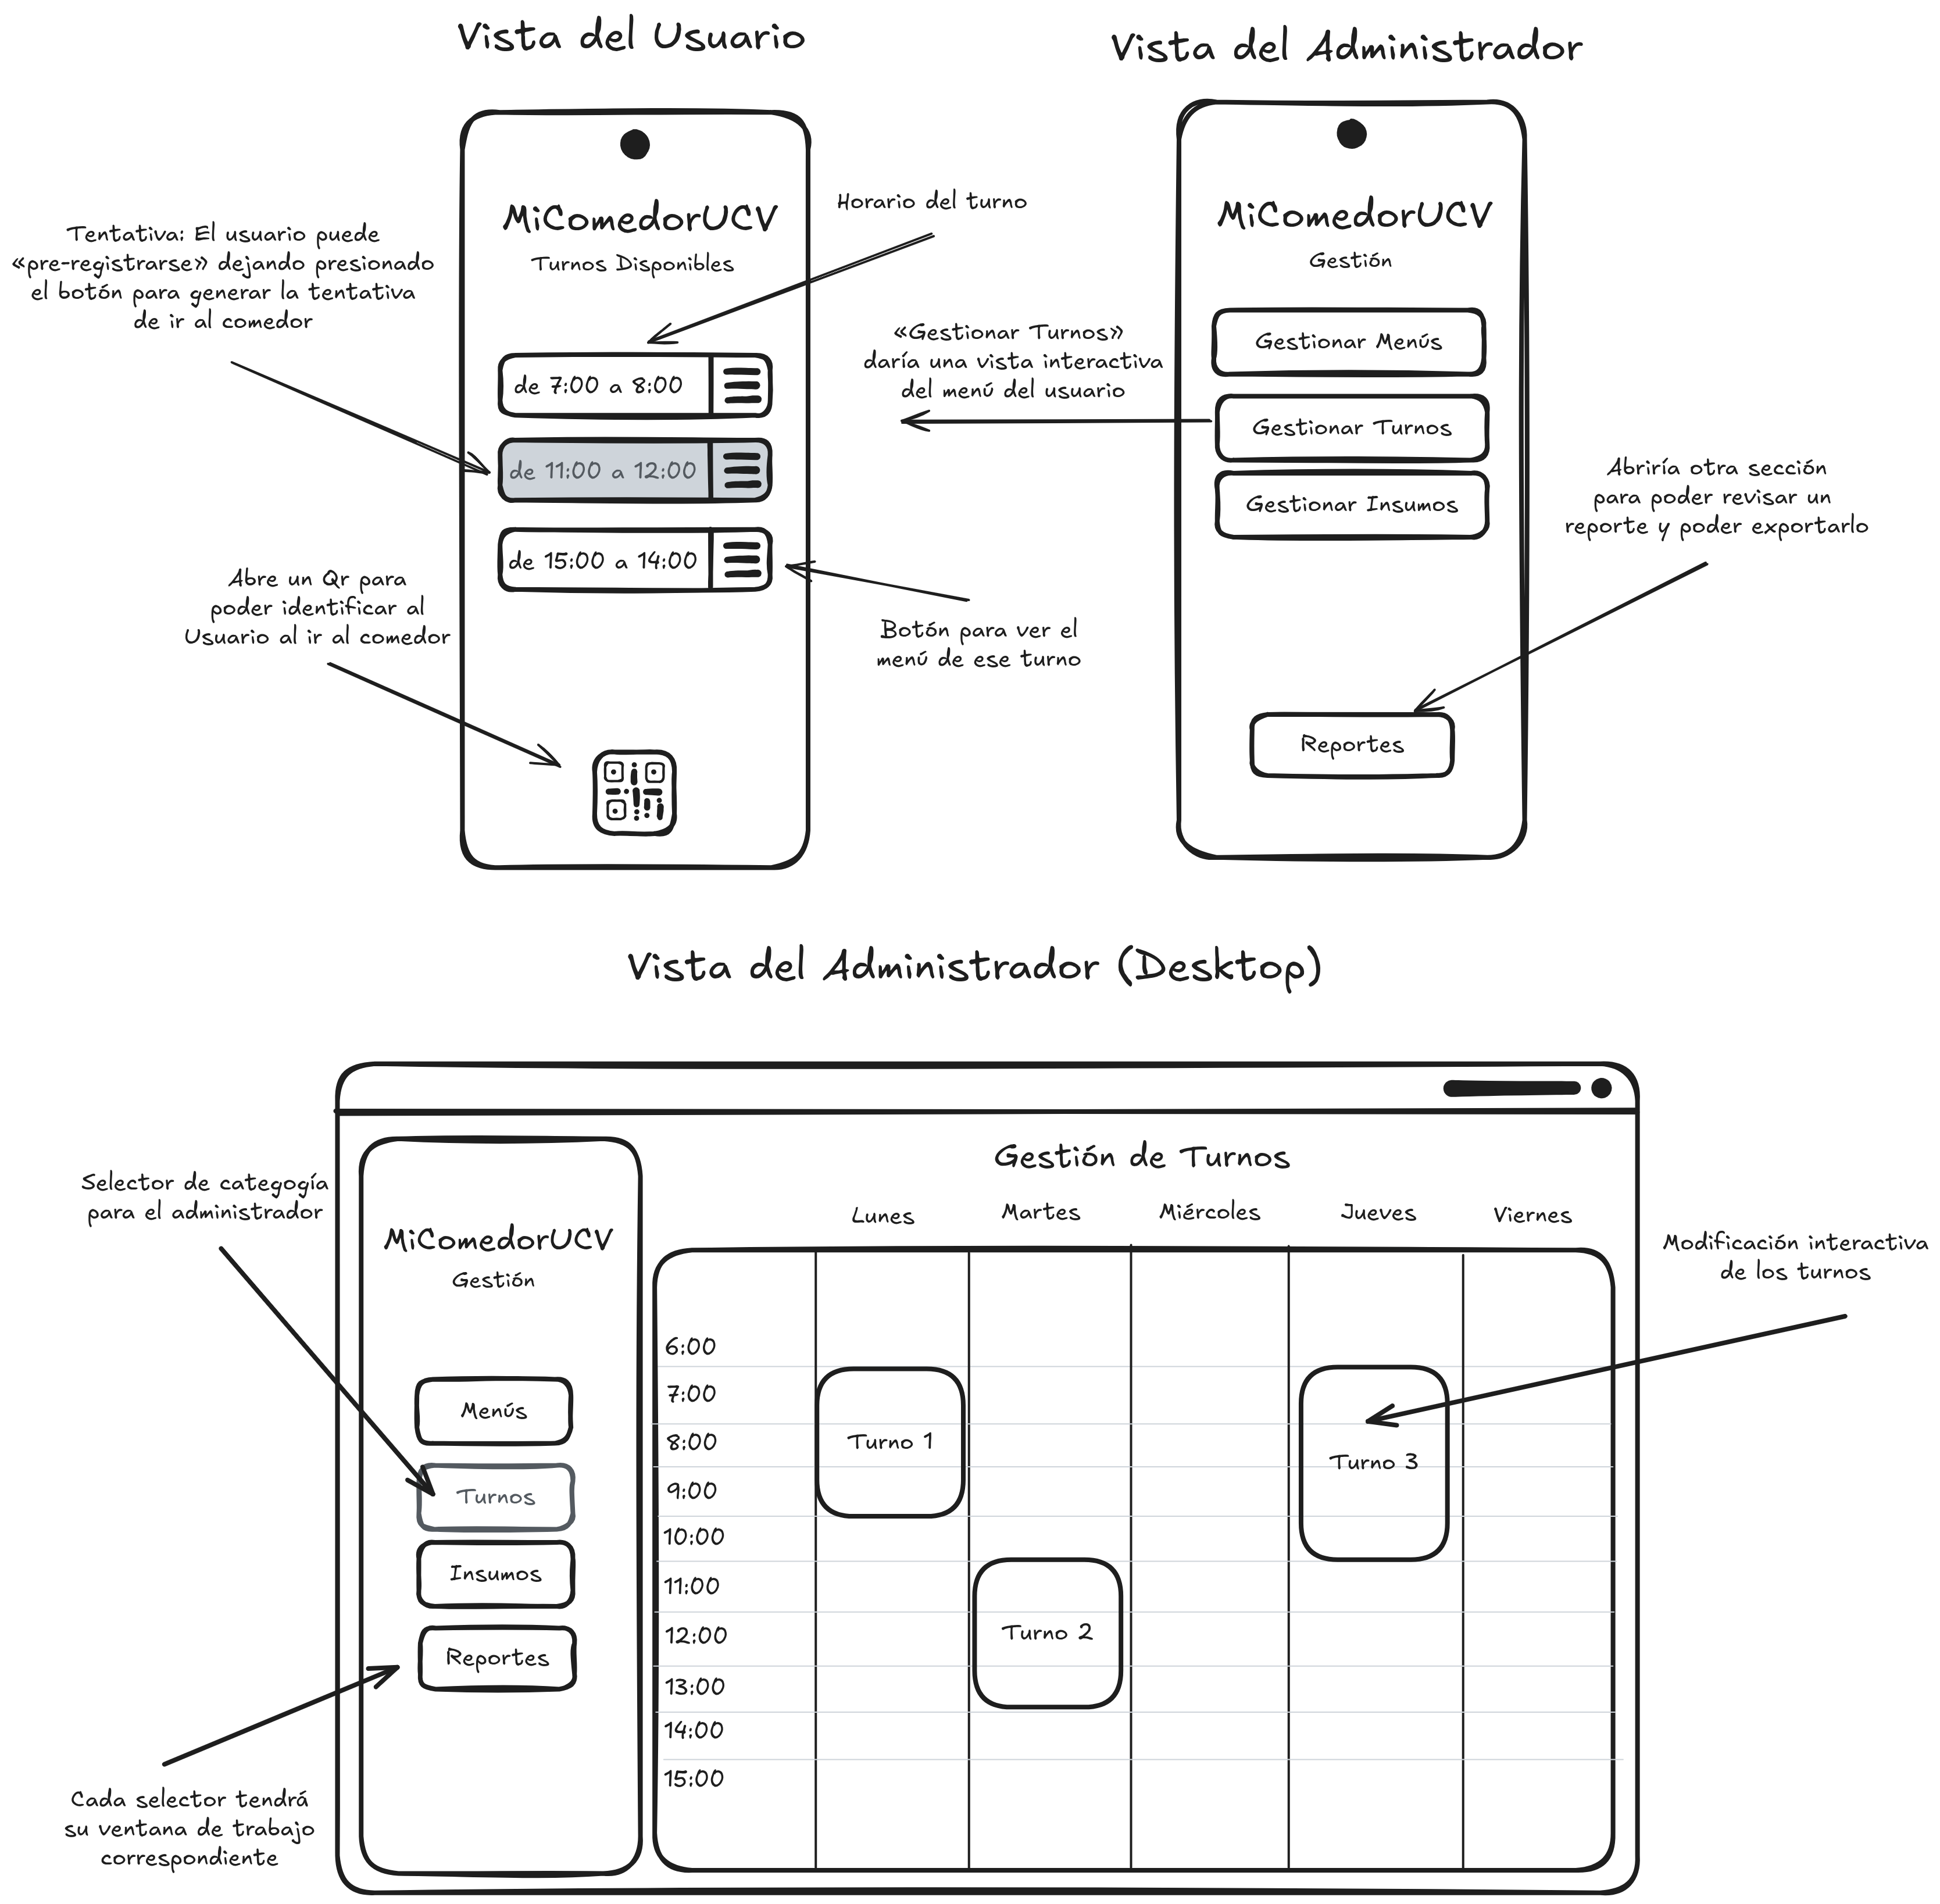
\includegraphics[width=16cm]{Requitements Discipline - Prototipe Wireframe.png}
\end{center}

\end{document}
